\section{Hardware}
\subsection{FLYSKY Receiver}
The FLYSKY receiver is a compact wireless communication module used in remote-controlled systems to receive control signals from a FLYSKY transmitter. It operates on a 2.4GHz frequency band and supports multiple channels, allowing it to control various actuators such as motors and servos. This receiver is widely used in drones, RC planes, and robots due to its reliable range, low latency, and compatibility with many FLYSKY models. It typically connects directly to a flight controller or electronic speed controller (ESC) for signal routing.
\begin{figure}
\centering
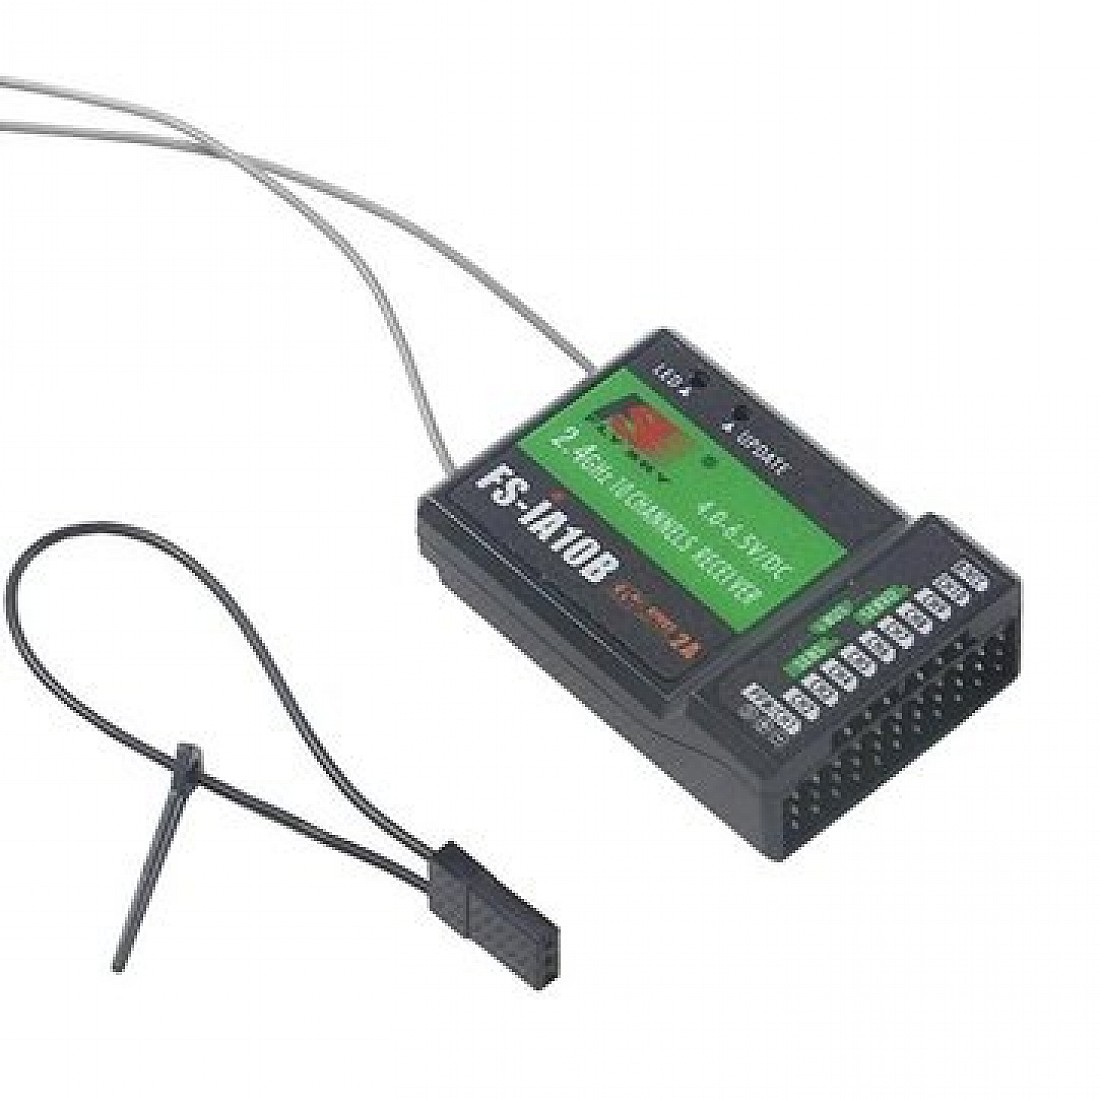
\includegraphics[width=0.5\textwidth]{images/flysky receiver.jpg}
\caption{Raspberry Pi 4 Model B}

\end{figure}

\subsection{30A ESC Skywalker}
The 30A Skywalker ESC (Electronic Speed Controller) is a device designed to control the speed, direction, and braking of a brushless motor. Rated for a maximum continuous current of 30 amps, it is ideal for medium-sized electric drones and RC aircraft. It takes signals from the receiver or flight controller and converts them into three-phase power for the motor, allowing smooth acceleration and precise speed control. The ESC also includes safety features like overheating and overcurrent protection.
\begin{figure}
\centering
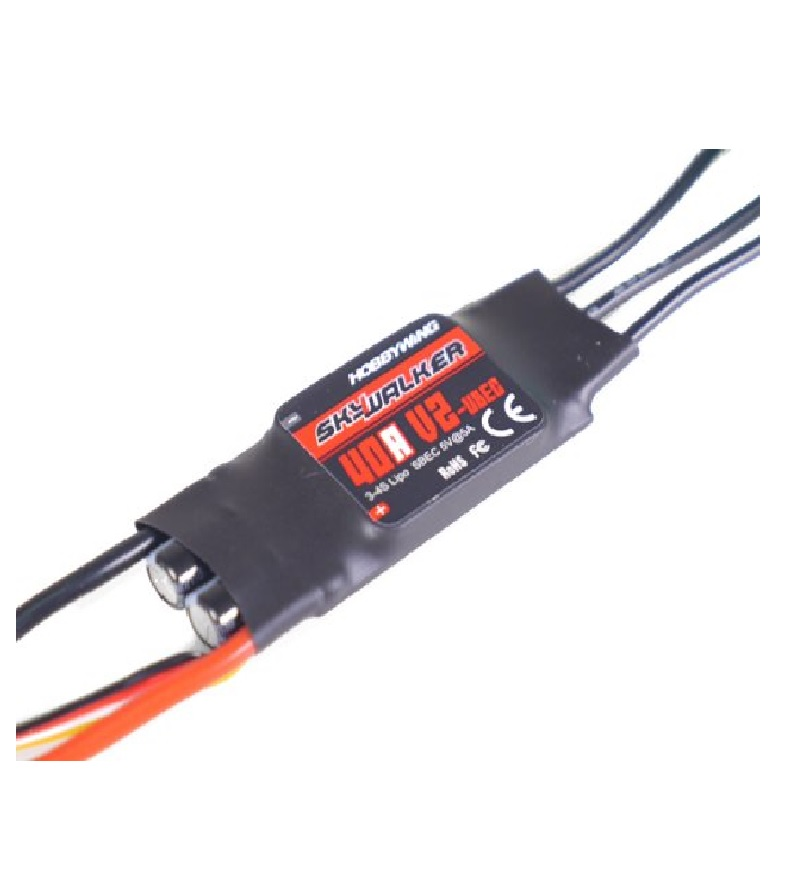
\includegraphics[width=0.5\textwidth]{images/esc.jpg}
\caption{Raspberry Pi 4 Model B}
\end{figure}

\subsection{Flight Stabilizer (NXE4 EVO)}
The NXE4 EVO Flight Stabilizer is an advanced control system used in RC aircraft and drones to maintain stability during flight. It uses onboard sensors such as gyroscopes and accelerometers to detect orientation and movement, and then automatically adjusts control surfaces or motor speeds to correct any deviations. This improves flight performance, especially in windy or unstable conditions, and enables smoother operation for both beginners and experienced pilots. It's essential for autonomous or semi-autonomous flight control.

\subsection{1000KV Brushless Motor}
A 1000KV brushless motor is a high-efficiency electric motor that rotates at 1000 revolutions per minute per volt applied. It is commonly used in drones, RC aircraft, and electric vehicles due to its power-to-weight ratio, reliability, and minimal maintenance needs. Unlike brushed motors, brushless motors have no internal contact between the rotor and stator, reducing wear and increasing lifespan. The motor typically has three wires for connection to an ESC and is paired with a propeller or gear mechanism for motion output.

\subsection{MG996 Metal Gear Servo}
The MG996 is a high-torque, metal gear servo motor used for precise angular movement in robotics, RC vehicles, and automation systems. Its durable metal gear construction offers increased torque and strength compared to plastic gear servos, making it suitable for demanding applications. Controlled by a PWM signal, it can rotate to specific angles between 0° and 180°, making it ideal for steering mechanisms, robotic arms, or flaps in RC aircraft. It comes with a standard 3-wire connector for power, ground, and signal.

\subsection{2200mAh 3S LiPo Battery}
The 2200mAh 3S LiPo (Lithium Polymer) battery is a high-capacity, lightweight power source commonly used in RC models, drones, and portable electronics. With three cells in series, it delivers a nominal voltage of 11.1V and a high discharge rate to support power-hungry components like motors and servos. Its 2200mAh capacity provides moderate runtime, making it ideal for short to medium-duration flights or robotic operations. The battery typically features a discharge plug (like XT60) and a balance connector for safe charging.

\subsection{Buck Module Voltage Regulator}
A buck module voltage regulator is a DC-DC converter that steps down higher input voltage to a lower, stable output voltage. It is commonly used in embedded electronics to power microcontrollers, sensors, and other 5V or 3.3V devices  from higher-voltage sources like LiPo batteries. The module includes components such as an inductor, capacitor, and adjustable potentiometer to maintain a consistent output. Its compact size and efficiency make it essential for battery-powered projects to protect components from over-voltage.

\subsection{Raspberry Pi with USB Camera and HDMI Cable}
The Raspberry Pi is a credit card-sized single-board computer capable of running a full Linux OS and performing various computing tasks. When paired with a USB camera, it can capture images and video for applications like computer vision, surveillance, and robotics. The HDMI cable allows video output to a monitor or display, enabling real-time viewing or debugging. This setup is ideal for lightweight, portable embedded systems where processing power, camera input, and display output are all required.
\begin{figure}
\centering
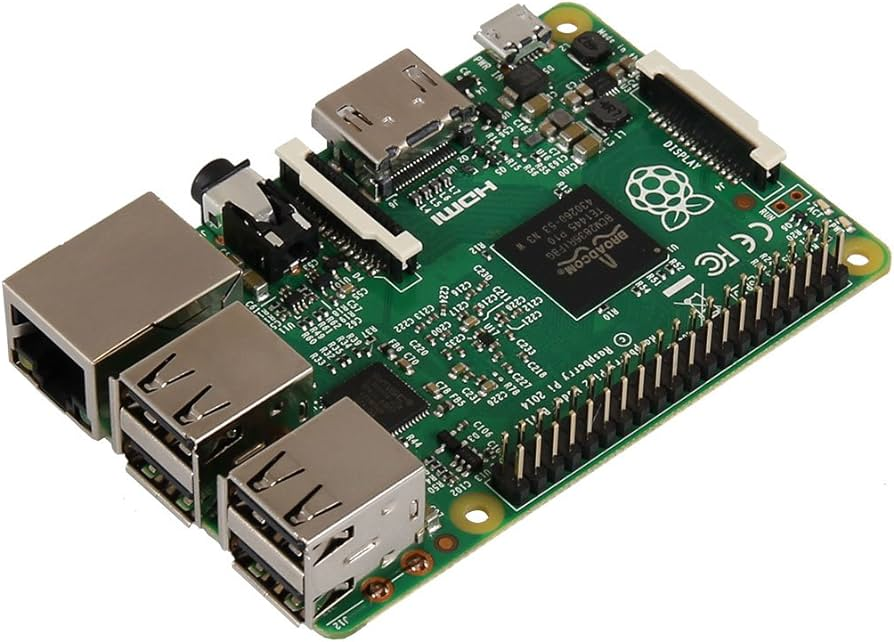
\includegraphics[width=0.5\textwidth]{images/raspimg.jpg}
\caption{Raspberry Pi 4 Model B}

\end{figure}

\section{Software Overview}

\subsection{ESRGAN for Image Super-Resolution}
\begin{figure}[H]
    \centering
    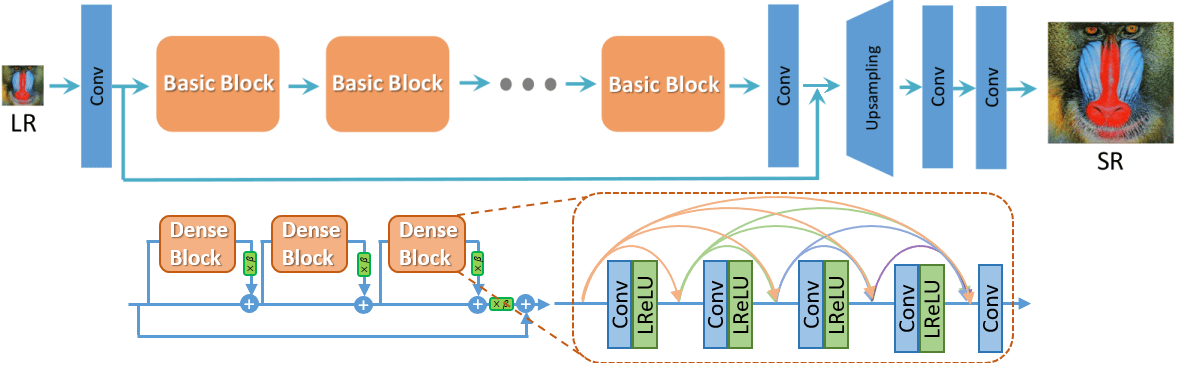
\includegraphics[width=0.85\linewidth]{images/esrganarchi.png}
    \caption{ESRGAN Architecture with Residual-in-Residual Dense Blocks (RRDB)}
    \label{fig:esrgan}
\end{figure}
ESRGAN introduced by Wang \emph{et al.} in 2018 [1], improves upon SRGAN by employing a deep generator built from Residual‑in‑Residual Dense Blocks (RRDB) without batch normalization. Each RRDB combines multiple convolutional layers, local dense connections, and global residual links to capture complex image features. The generator upsamples low‑resolution inputs (e.g.\ 820×616 pixels) by a factor of 4× to high‑resolution outputs (e.g.\ 3280×2464 pixels). The discriminator is relativistic, estimating the probability that a real image is more realistic than a generated one, which enhances stability and visual fidelity. ESRGAN further integrates a perceptual loss based on high‑level VGG features computed before ReLU activations, preserving fine textures and brightness consistency. This design enables ESRGAN to produce photorealistic details, as demonstrated by its victory in the PIRM2018 SR Challenge [1].

In our UAV system, images captured onboard with a Raspberry Pi USB Camera are retrieved post‑flight. ESRGAN runs on a ground PC to upscale extracted frames, recovering critical details (e.g.\ building outlines, vegetation patterns) necessary for accurate land use classification in the Kathmandu region.

\subsection{Comparison of Super-Resolution Models}
We compare ESRGAN with earlier SR approaches:

\begin{table}[H]
\centering
\renewcommand{\arraystretch}{1.2}
\setlength{\tabcolsep}{6pt}
\begin{tabular}{@{} l l p{3cm} p{3cm} p{3cm} @{}}
    \toprule
    \textbf{Model} & \textbf{Year} & \textbf{Architecture} & \textbf{Strengths} & \textbf{Weaknesses} \\
    \midrule
    SRCNN   & 2014 & 3-layer CNN & Simple, fast & Overly smooth outputs [2] \\
    FSRCNN  & 2016 & CNN + deconv & Efficient, higher PSNR [2] & Limited texture detail \\
    EDSR    & 2017 & Deep ResNet & High PSNR, faster [3] & Less perceptual quality \\
    ESRGAN  & 2018 & GAN + RRDB & Realistic textures, sharp edges [1] & Computationally intensive \\
    \bottomrule
  \end{tabular}
  \caption{Comparison of Super-Resolution Models}
\label{tab:sr_models}
\end{table}


\subsection{Land Use Classification}
Land use classification from UAV imagery entails categorizing pixels or patches into classes such as forest, agriculture, water, and urban. Common approaches include:
\begin{itemize}
  \item \textbf{Convolutional Neural Networks (CNNs)}: End‑to‑end models (e.g.\ U‑Net, ResNet, EfficientNet) that learn spatial hierarchies directly from upscaled images [4].
  \item \textbf{Random Forest (RF)}: Ensemble of decision trees trained on raw pixels or derived indices, robust to overfitting and effective for moderate datasets [2,4].
  \item \textbf{Support Vector Machine (SVM)}: Kernel‑based classifier suitable for moderate‑sized, well‑separated classes [2,4].
\end{itemize}
A hybrid approach often combines CNN feature extractors with RF or SVM classifiers, leveraging deep networks for hierarchical feature learning and traditional ML for robust classification when labeled data is limited.

\subsection{Software}
The software pipeline integrates the following tools and libraries:
\begin{itemize}
  \item \textbf{OpenCV}: For image/frame extraction, filtering, and geometric transformations [5].
  \item \textbf{NumPy \& SciPy}: Core numerical and array operations for preprocessing.
  \item \textbf{scikit-learn}: Implements RF and SVM classifiers, data splitting, scaling, and evaluation utilities [6].
  \item \textbf{TensorFlow \& PyTorch}: Deep learning frameworks for ESRGAN and CNN implementation. PyTorch (BasicSR toolkit) eases experimentation [7], while TensorFlow (TF‑Hub ESRGAN) supports scalable deployment [8].
  \item \textbf{GDAL/Rasterio}: For handling geo-referenced imagery and aligning with regional GIS data [9].
\end{itemize} 


\subsection{Dataset}

\textbf{1. Kathmandu Land Use Datasets}

Region-specific datasets used for land use classification in Kathmandu:

\begin{itemize}
  \item \textbf{Nepal National Land Cover Dataset}: Annual land-cover maps (2000–2022) from Landsat imagery via Google Earth Engine, covering forests, agriculture, water, and built-up areas[10].
  \item \textbf{Kathmandu City Land Use Shapefiles}: Urban land use polygons (residential, commercial, parks) for Kathmandu Metropolitan City (2011) from ICIMOD[11].
  \item \textbf{OpenStreetMap Polygons}: Land-use tags for Kathmandu accessible through the Humanitarian Data Exchange[12].
\end{itemize}

\textbf{2. Image Super-Resolution Datasets}

Datasets used to train and evaluate ESRGAN and other super-resolution models:

\begin{itemize}
  \item \textbf{DIV2K}: A large-scale dataset designed for image super-resolution, consisting of 1000 high-resolution images and their corresponding low-resolution counterparts. Suitable for training deep SR models.
  \item \textbf{Set5 and Set14}: Benchmark datasets commonly used for evaluating the performance of super-resolution models. While smaller in size, they are widely adopted for quantitative comparisons.
\end{itemize}

These datasets provide essential ground truth for training and validating both our land use classification pipeline and image super-resolution models.

